\documentclass[sans]{beamer}

\mode<presentation>
{
	% \usetheme{CambridgeUS}
	% \usetheme{Hannover}
	\usetheme{Singapore}
	\usecolortheme{default}
}

\usepackage{cmap}
\usepackage{listings}
\usepackage{lmodern}
\usepackage{color}
\usepackage{minted}
\usepackage{graphicx}
\usepackage{tikz}
\usetikzlibrary{arrows}
\usepackage{wrapfig}
\usepackage{bussproofs}
\usepackage{stmaryrd}

\usepackage[labelformat=empty]{caption}
\usepackage{fontspec}
% \usepackage{polyglossia}
% \setdefaultlanguage{russian}

% \setmainfont[Ligatures=TeX]{DejaVu Serif}
% \setsansfont[Ligatures=TeX]{DejaVu Sans}
% \setmonofont{DejaVu Sans Mono}

\definecolor{myGray}{RGB}{50,50,50}
\EnableBpAbbreviations

\begin{document}

\title
[Concurrency Control]
{Concurrency Control: Methods, Performance, and Analysis}

\subtitle{Based on Alexander Thomasian paper}

\author
[Podkopaev]{Anton Podkopaev, podkoav239@gmail.com}
\institute{SPbSU}
\date [21-11-14]{21 nov 2014}

\begin{frame}[plain]
	\titlepage
\end{frame}

\section{Introduction}

\begin{frame}{Main Line}
  \begin{itemize}
    \item Comparison of locking methods

    \item Sources of performance degradation with standard locking:
      \begin{itemize}
        \item Blocking
        \item Deadlock
      \end{itemize}

    \item Restart-oriented locking methods
    \item Waith-depth-limited (WDL) methods

    \item Restart waiting
  \end{itemize}
\end{frame}

\begin{frame}{Notions}
  \begin{itemize}
    \item Work only with correctness criterion as serializability
    \begin{itemize}
      \item It isn't suitable for systems like trading bids
    \end{itemize}
    
    \item Strict 2PL
    \begin{itemize}
      \item Locks to be released only when the txn is
            commited or aborted
      \item To solve cascading aborts
    \end{itemize}

    \item Work only with centralized high-performance systems
  \end{itemize}
\end{frame}

\begin{frame}{Method Sets}
  \begin{itemize}
    \item Restart-oriented locking
    \begin{itemize}
      \item Wait-depth-limited (WDL)
    \end{itemize}

    \item Two-phase processing methods
    \begin{itemize}
      \item Txn re-execution may not require disk I/O
            in case of big buffer
    \end{itemize}
    \item Optimistic CC (OCC)
    \begin{itemize}
      \item Viable for two-phase processing
    \end{itemize}
    \item Time-stamp ordering (TSO)
    \begin{itemize}
      \item For distributed databases
    \end{itemize}
  \end{itemize}
\end{frame}

\section{Model}

\begin{frame}{Hardware and Data Resource Contention}
  \begin{itemize}
    \item Hardware contention
    \begin{itemize}
      \item The primary effect on performance
    \end{itemize}
    \item Data contention
    \begin{itemize}
      \item The secondary effect
    \end{itemize}
  \end{itemize}
\end{frame}

\begin{frame}{Transaction Structure}
  \begin{itemize}
    \item Considering
      \begin{itemize}
        \item Only flat txns
        \item Mostly short update transactions
      \end{itemize}

    \vfill

    \item A txn accessing $k$ objects consists of
      $k + 1$ steps ($C_k$ --- class of txn)
    \item Each step involves CPU processing and disk accesses
    \item After last step --- \emph{commit}
    \begin{itemize}
      \item Locks held by txn are released
    \end{itemize}

  \end{itemize}
\end{frame}

\begin{frame}{Transaction Arrival Process}
  \begin{itemize}
    \item $S$ --- a number of sources
    \item $Z$ --- a think time
    \item $M$ --- a number of txn already at the system
    \vfill
    \item $\Lambda(M) = (S - M)/Z$ --- the arrival rate

    \vfill
    \item \emph{The user isn't involved after the txn is submitted}
  \end{itemize}
\end{frame}

\begin{frame}{System Categories}
  \begin{itemize}
    \item \emph{Open} system --- sufficently large $S$
    \begin{itemize}
      \item The \emph{mean response time characteristic} can be used for the
            performance comparison of CC methods
    \end{itemize}
    \item \emph{Closed} system --- $S = M$ and $Z = 0$
    \begin{itemize}
      \item Can be used to estimate the peak performance of CC methods
      \item Throughput $T(M), M \geq 1$ 
    \end{itemize}
  \end{itemize}
\end{frame}

\begin{frame}{Frequency-based Model}
  \begin{itemize}
    \item The fraction $f_k$  of txns in $C_k$
    \vfill

    \item Open systems
    \begin{itemize}
      \item $\Sigma^K_{k = 1} f_k = 1, f_k \geq 0$
      \item The arrival rate $\lambda_k = \lambda f_k$
      \item $R_k$ --- the mean response time of txns in $C_k$
      \item The mean number of txns in $C_k$ is $M_k = \lambda_kR_k$
    \end{itemize}
    \vfill
    \item Closed systems
    \begin{itemize}
      \item $M_k$ --- transaction concurrency in $C_k$
      \item Immediately relacing of txn in $C_k$ with probability $f_k$
      \item Throughput in $C_k$ --- $T_k(M) = f_k T(M)$
    \end{itemize}
  \end{itemize}
\end{frame}

\begin{frame}{Database Access Model}
  \begin{itemize}
    \item The \emph{granule} --- the unit of data at which CC is applied to the DB
    \begin{itemize}
      \item Page-level \emph{or} Record-level lock
    \end{itemize}
    \item $D$ --- a number of objects in the DB
    \item DB objects are accessed with probabilities
    \begin{itemize}
      \item In most studies --- uniform probability
      \item Another way --- the hot-spot model, $b$ -- $c$ rule 
    \end{itemize}
  \end{itemize}
\end{frame}

\begin{frame}{Computer System Model (1)}
  \begin{itemize}
    \item A queueing network model (QNM)
    \item The CPU processing time --- txn path-length and CPU speed
    \item The disk processing time --- disk access time and the number of disk I/Os
    \item The infinite-resource model
    \begin{itemize}
      \item Useful in comparing the performance limits of CC methods
      \item Each txn has its own virtual CPU and execution time is independent of concurrent txns
    \end{itemize}
    \item The finite-resource model
    \begin{itemize}
      \item Important in case of comparision restart-oriented CC methods with blocking-oriented ones
    \end{itemize}
  \end{itemize}
\end{frame}

\begin{frame}{Computer System Model (2)}
  \begin{columns}

  \begin{column}{.5\linewidth}
    \begin{itemize}
      \item $p_0$ --- a probability of success at current tick
      \item $P_k = p_0 (1 - p_0)^{k - 1} \approx 1/p_0$
      \item $p_n$ --- a probability of access $n$th disk
      \item The number of $n$th disk visits --- $p_n/p_0$
    \end{itemize}
  \end{column}
  \begin{column}{.6\linewidth}
    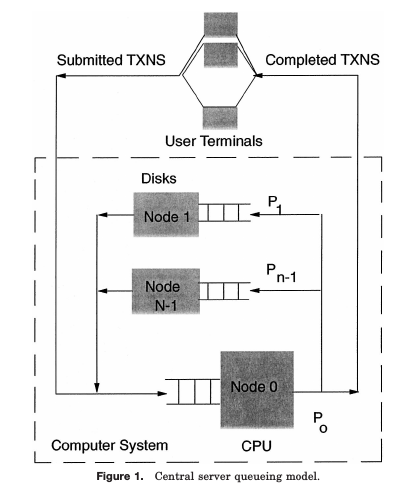
\includegraphics[width = \linewidth]{images/qnmScheme.png}
  \end{column}

  \end{columns}
\end{frame}


\begin{frame}{Computer System Model (3)}
  \begin{itemize}
    \item Product form QNM
    \item Hierarchical solution method
  \end{itemize}
\end{frame}

\begin{frame}{Performance Degradation due to CC Methods}
  \begin{itemize}
    \item No (or negligible) wasted processing
      \begin{itemize}
        \item $T(M) \approx t(M_a)$
      \end{itemize}
    \item Restarts but no blocking
      \begin{itemize}
        \item The system efficiency --- $T(M) / t(M)$
      \end{itemize}
    \item Blocking and restarts
      \begin{itemize}
        \item The system efficiency --- $T(M_a) / t(M_a)$
      \end{itemize}
  \end{itemize}
\end{frame}

\begin{frame}{Separation of Hardware and Data-resource Contention}
  \begin{itemize}
    \item Desirable property --- allows the system-throughput characteristic (STC) to be computed only once
    \item Possible in case of insignificant or independent of the level of lock data contention overhead
  \end{itemize}
\end{frame}

\section{Standard Locking}

\section{Restart-Oriented Locking}

\section{Two-phase Processing}

\section{Conclusion}

\end{document}
